% siminos/atlas/cut.tex  pdflatex atlas
% $Author$ $Date$

\section{Sections}
\label{s:cut}

% Predrag's original text:
%In the {\em Poincar\'e section} method one records the coordinates of the
%trajectory $\ssp(\zeit)$ at the instant $\sspRed_n = \ssp(\zeit_n)$ \DB{\color{red} Don't like %the notation here since $t_N$ has already been introduced in \reffig{fig:A27wurst} for group %tangent vectors.  The difference is kind of subtle.}
%it traverses the fixed oriented hypersurface $\PoincS$ of
%codimension 1. 


In the {\em Poincar\'e section} method one records the coordinates $\sspRed_n$ of the
trajectory $\ssp(\zeit)$ at the instants $\zeit_n$ when it traverses a fixed oriented hypersurface $\PoincS$ of codimension 1. For high-dimensional flows that we have in mind, the
practical choice is a hyperplane, the type of Poincar\'e section (or,
from now on, just a \emph{section})  we shall consider here. Such a
section captures important features of the flow in an open neighborhood
of the section-fixing \template. \DB{2012-04-12}{\color{red} Not a huge fan of $t_n$. It could be confused with $t_N$. Kinda subtle.}

%%%%%%%%%%%%%%%%%%%%%%%%%%%%%%%%%%%%%%%%%%%%%%%%%%%%%%%%%%%%%%%%%%%%%
\begin{figure}
  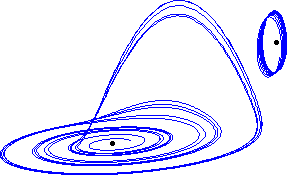
\includegraphics[width=0.3\textwidth]{RoessTrjs}
    \caption{
R\"ossler \eqva\ and their invariant manifolds. The stable manifold of
the inner {\eqv} $\ssp_{-}$  is 1-dimensional and the unstable one is a
spiral-out focus. For the outer {\eqv} $\ssp_{+}$  the stable manifold is
a spiral-in focus (basin boundary for initial conditions that either fall
into the chaotic attractor, or escape to infinity) and the unstable
manifold is 1-dimensional.
    }
\label{fig:RoessTrjs}
\end{figure}
%%%%%%%%%%%%%%%%%%%%%%%%%%%%%%%%%%%%%%%%%%%%%%%%%%%%%%%%%%%%%%%%%%%%%

As an example consider the system of R\"ossler\rf{ross},
\index{R\"ossler system}
\beq
\begin{split}
  \dot{x} &= -y \,-\,z \\
  \dot{y} &= x + a y \\
  \dot{z} &= b + z (x - c)
  \,,
  \label{eq:Rossler}
\end{split}
\eeq
where $a = b = 0.2$ and $c = 5.7$. This flow has two prominent invariant
states, the `inner' and the `outer' unstable \eqva\ ($\ssp_{-}$  and $\ssp_{+}$) which we pick as {\em \template s} (\refFig{fig:RoessTrjs}). \DB{2012-04-12}{\color{red}Since we are using them as section templates, should the equilibria be called $\hat{x}'_{\pm}$ for consistency?}

We orient the sections so the plane $\PoincS_{-}$ contains the 1\dmn\
stable eigenvector (\reffig{fig:RoessNearEq}) of $\ssp_{-}$, and the other section
$\PoincS_{+}$ contains the 1\dmn\ unstable eigenvector of $\ssp_{+}$
(\reffig{fig:RoessFarEq}), thus capturing the local spiral-in,
spiral-out dynamics. The remaining freedom to rotate each section can be
used to orient them in such a way that the ridge (the intersection of
the two sections) lies approximately halfway between the two templates
(\reffig{fig:RoessBothEq}).

A well chosen section captures the dynamics in the neighborhood of its
\template, but how far does this neighborhood extend?
The answer is that the section captures neighboring trajectories as long
as it cuts them transversally; it fails the moment the velocity field at 
a point $\sspRSing$ fails to pierce the section. At these locations, the
velocity either vanishes (\eqv) or is tangent to the section, \ie,
orthogonal to the section normal $\hat{n}$,
\beq
    \hat{n} \cdot \vel(\sspRSing) = 0
\,,\qquad
    \sspRSing \in \cal{S}
\,.
\ee{eq:sspRSing}
For a smooth flows such points form a smooth $(d\!-\!2)$\dmn\
\emph{\poincBord} ${\cal S} \subset \PoincS$, which encompasses the open
neighborhood of the {\template} characterized by qualitatively similar
flow. We shall refer to this region of the section as a
`chart' of the {\template} neighborhood (see figures \reffigs{fig:RoessNearEq}{fig:RoessFarEq}). Beyond the border, the flow pierces the section hyperplane in the `wrong' direction and the dynamics are qualitatively different.


%%%%%%%%%%%%%%%%%%%%%%%%%%%%%%%%%%%%%%%%%%%%%%%%%%%%%%%%%%%%%%%%%%%%%
\begin{figure}%[H]
\begin{center}
  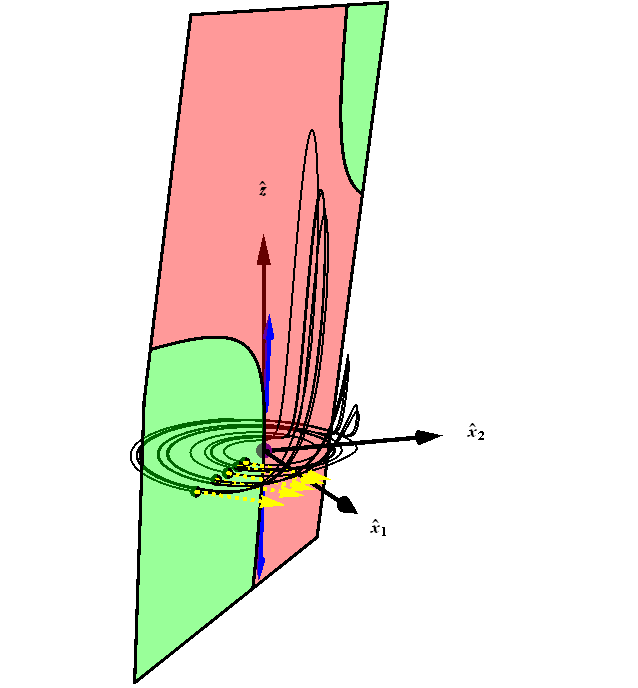
\includegraphics[width=0.30\textwidth,clip=true]{RoessNearEq2}
\end{center}
  \caption{\label{fig:RoessNearEq}
  A R\"ossler flow Poincar\'e section $\PoincS_{-}$ through the inner
  {\eqv} $\ssp_{-}$ and its stable eigenvector. The green region highlights the chart of the $\ssp_{-}$ neighborhood.
}
\end{figure}
%%%%%%%%%%%%%%%%%%%%%%%%%%%%%%%%%%%%%%%%%%%%%%%%%%%%%%%%%%%%%%%%%%%%%

%%%%%%%%%%%%%%%%%%%%%%%%%%%%%%%%%%%%%%%%%%%%%%%%%%%%%%%%%%%%%%%%%%%%%
\begin{figure}%[H]
\begin{center}
  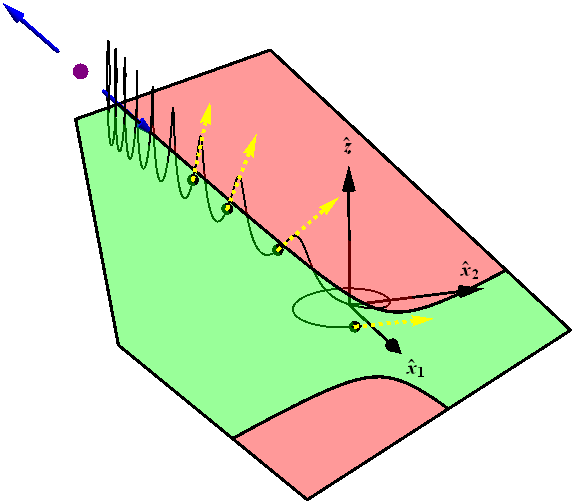
\includegraphics[width=0.30\textwidth,clip=true]{RoessFarEq2}
\end{center}
  \caption[R\"ossler section, outer {\eqv}]{
  A Poincar\'e section for R\"ossler flow
      through the
      outer
  {\eqv} $\ssp_{+}$  and its unstable eigenvector. The green region highlights the chart of the $\ssp_{+}$ neighborhood.
  } \label{fig:RoessFarEq}
\end{figure}
%%%%%%%%%%%%%%%%%%%%%%%%%%%%%%%%%%%%%%%%%%%%%%%%%%%%%%%%%%%%%%%%%%%%%

%%%%%%%%%%%%%%%%%%%%%%%%%%%%%%%%%%%%%%%%%%%%%%%%%%%%%%%%%%%%%%%%%%%%%
\begin{figure}%[H]
\begin{center}
  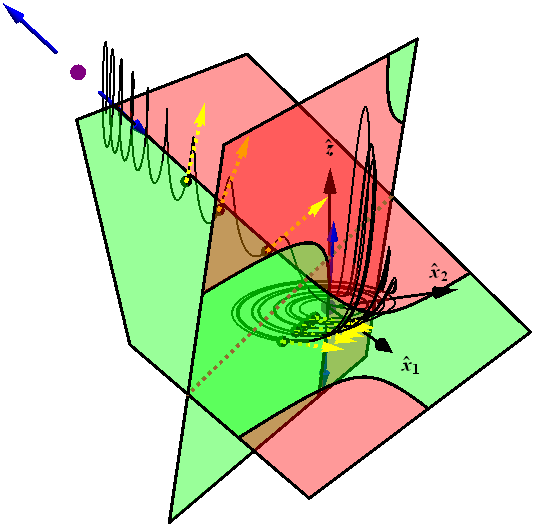
\includegraphics[width=0.30\textwidth,clip=true]{RoessSctAtlas2}
\end{center}
  \caption{
  A two-section atlas for R\"ossler flow, with the local sections of
  \reffigs{fig:RoessNearEq}{fig:RoessFarEq} oriented and combined so that
  the ridge (intersection of the two sections, indicated by the dotted brown
  line) lies  approximately midway between the \template s.
  } \label{fig:RoessBothEq}
\end{figure}
%%%%%%%%%%%%%%%%%%%%%%%%%%%%%%%%%%%%%%%%%%%%%%%%%%%%%%%%%%%%%%%%%%%%%

%\subsection{R\"ossler two-chart atlas}

For R\"ossler flow \refeq{eq:Rossler}, ${\cal S}$ \refeq{eq:sspRSing} is given by a
quadratic condition in 3 dimensions, so \poincBord\ is a conic section as
drawn in \reffigs{fig:RoessNearEq}{fig:RoessFarEq}. The two
charts meet at a ridge, and together do a pretty good job as the 2-chart
atlas of the interesting R\"ossler dynamics, \reffig{fig:RoessBothEq}. As
explained in ChaosBook.org\cite{DasBuch}, due to extreme contraction rate, the section
in \reffig{fig:RoessNearEq} is for all practical purposes 1\dmn, and the
associated return map yields all \po s of the 3\dmn\ flow.

In 3 dimensions everything -sections, ridges, \poincBord s-  can be
drawn. But what about high-dimensional flows? The point is that while it
is impossible to visualize  $(d\!-\!2)$\dmn\ {\poincBord}, a point is a
point, and a line is a line in a projection from any number of
dimensions, so a trajectory crossing of both a section and a {\poincBord}
can be easily determined and visualized in any dimension.

% \subsection{$N$-chart atlas, forward maps}
% \subsection{Ring of Fire return map\rf{lanCvit07}}

To summarize: we can chart a region of \statesp\ of interest, by a
picking a sufficient number of \template s and their associated charts,
each bounded by \poincBord s and ridges.

Two concluding remarks on what sections \emph{are not}:

(1) A Poincar\'e section is {\em not} a projection onto a
lower-dimensional space: Rather, it is a local change of coordinates to a
direction along the flow, and the remaining coordinates transverse to it.
No information about the flow is lost; the full space trajectory can
always be reconstructed by integration from a point in the section.

(2) The method of Poincar\'e sections is {\em not} equivalent to
\emph{strobing} a flow at a sequence of instants in time. While
`strobing' is what any numerical integrator does, by representing a
trajectory by a sequence of time-integration step separated points,
strobing is in general not a reduction of a flow to a codimension 1
manifold, as the sequence of strobed points still resides in the full
\statesp\ $\pS$, of dimensionality $d$.
